\documentclass[letter,11pt]{article}
\usepackage[pdftex]{graphicx}
\usepackage{float}
\begin{document}
	\begin{center}
		\Large\textbf{CDCI 567-Machine Learning Assignment-1}
	\end{center}
	
	\section{Density Estimation}
	\subsection{MLE}
	\subsubsection{Beta($\alpha$,1)}
	$x_{1},x_{2},...,x_{n}$ are samples of $Beta(\alpha,1)$ distribution.
	
	In this case, pdf of $x_(i), i=1,...,n$ is $$f(x_{i}|\alpha,1))=\frac{x^{\alpha-1}}{\beta(\alpha,1)}=
	\frac{x^{\alpha-1}}{\int_{0}^{1}t^{\alpha-1}dt}=
	\alpha x^{\alpha-1}$$
	
	Likelihood function and log likelihood function:
	$$L(\alpha,1|x)=\prod_{i=1}^{n}\alpha x^{\alpha-1}$$
	$$l(\alpha,1|x)=log(\alpha^{n}) + log(\prod_{i=1}^{n}x_{i}^{\alpha-1})=
	nlog(\alpha) + \sum_{i=1}^{n}(\alpha-1)log(x_{i})$$
	
	Derivative of $l(\alpha,1|x)$:
	$$\frac{\partial l(\alpha,1|x)}{\partial \alpha} = \frac{n}{\alpha} + \sum_{i=1}^{n}log(x_{i})=0$$
	
	$$\frac{\partial^{2} l(\alpha,1|x)}{\partial \alpha} = -\frac{n}{\alpha^{2}} < 0$$
	
	$$\hat{\alpha} = -\frac{n}{\sum_{i=1}^{n}log(x_{i}}$$
	\subsubsection{Normal($\theta$,diag($\theta$))}
	$x_{1},x_{2},...,x_{n}$ are samples of $Normal(\theta,diag(\theta))$ distribution.
	In this case, pdf of $x_{i}, i = 1,...,n$ is
	$$f(x_{i}|\theta,diag(\theta)) = \frac{1}{\sqrt{2\pi diag(\theta})}\exp(-\frac{(x_{i}-\theta)}{2\theta})$$
	
	Likelihood function and log likelihood function:
	$$L(\theta,diag(\theta)|x_{i}) = (2\pi)^{-\frac{d}{2}}|diag(\theta)|^{-\frac{1}{2}}\exp(-\frac{1}{2}(x-\theta)^{T}diag(\theta)^{-1}(x-\theta))$$	
	
	$$|diag(\theta)| = \theta^{d}$$
	$$l(\theta,diag(\theta)|x_{i}) = -\frac{d}{2}log(2\pi\theta) - \sum_{i=1}^{n}\frac{1}{2} \frac{(x_{i}-\theta_{i})^{T}(x_{i}-\theta_{i})}{\theta_{i}}$$
	
	Derivative of $l(\theta,diag(\theta)|x_{i})$:
	$$\frac{\partial l(\theta,diag(\theta)|x_{i})}{\partial \theta} = -\frac{dn}{2\theta} - \frac{n}{2} + \frac{1}{2\theta^{2}}\sum_{i=1}^{n}x_{i}^{2} = 0$$
	
	$$\hat{\theta} = -\frac{d}{2} + \frac{1}{2}\sqrt{d+\frac{4}{n}\sum_{i=1}^{n}x_{i}^{2}}$$
	\subsection{MLE in Linear Regression}
	\subsubsection{$w_0$ and $w$}
	According to lecture pdf:
	
	$$logP(D) = -\frac{1}{2}(\frac{1}{\sigma^2}\sum_{n}^{}[y_n-(w_0+w^Tx_n)]^2)$$
	
	To maximize the log likelihood, we need to minimize:
	$$\sum_{n}^{}[y_n - (w_0+w^Tx_n)]^2 = \sum_{n}^{}[y_n^2-2y_nw_0-2y_nw^Tx_n+w_0^2+2w_0w^Tx_n+(w^Tx_n)^2]$$
	
$$\frac{\partial \sum_{n}^{}[y_n - (w_0+w^Tx_n)]^2}{\partial w_0} = -2\sum y_n + 2Nw_0+2\sum w^Tx_n = 0$$
	$$\hat{w_0} = \frac{\sum y_n - \sum w^Tx_n}{N} = \bar{y}-w^T\bar{x}$$
	
	$RSS(w)$ in matrix form:
	$$RSS(w) = \sum_{n}^{}[y_n-(w_0+w^Tx_n)]^2$$
	
	If we write $w_0$ equation found above:
	$$RSS(w) = \sum_{n}^{}[y_n-\bar{y}+w^T\bar{x}-w^Tx_n]$$
	
	Where $y_n - \bar{y} = y_c$ and $x_n - \bar{x} = x_c$:
	$$RSS(w) = \sum_{n}^{}[y_c-w^Tx_c]^2 = \sum_{n}^{}(y_c-w^Tx_c)(y_n-x_c^Tw)$$
	$$= \sum_{n}^{}w^Tx_cx_c^Tw-2y_cx_c^Tw+ const = {w^T(\sum_{n}^{}x_cx_c^T)w - 2(\sum_{n}^{}y_nx_c^T)w} + const$$
	
	$$RSS(w) = [w^TX_c^TX_cw-2(X_c^TY_c)^Tw]$$
	$$\frac{\partial RSS(w)}{\partial w} = X_c^TX_cw-X_c^TY_c = 0$$
	$$w^{LMS} =(X_c^TX_c)^{-1}X_c^TY_c$$
	
	\subsubsection{Conditional Gaussian}
	
	$[X,Y]$ is multivariate Gaussian distributed.
	
	
	
	\subsection{Kernel Density Estimation}
	Random variables $X_1,...,X_n$ are i.i.d. sampled from $f(x)$ function.
	
	$$E_{X_1,...,X_n}[\hat{f}(x)] = E[\frac{1}{nh}\sum_{i=1}^{n}K(\frac{x-t}{h})] = \frac{1}{nh}\sum_{i=1}^{n}E[K(\frac{x-t}{h})] =  \frac{1}{nh}nE[K(\frac{x-t}{h})]$$
	$$E_{X_1,...,X_n}[\hat{f}(x)] = \frac{1}{h} \int_{}^{}K(\frac{x-t}{h})f(t)dt$$
	
	$$f(x-hz) = f(x) + f'(x)(x-hz-x)+\frac{f''(x)}{2!}(x-hz-x)^2 + ...+\frac{f^k(x)}{k!}(x-hz-x)^k+h_k(x-hz)(x-hz-x)^k$$
	
	$z = \frac{x-t}{h}$ which means $t = x - hz$
	
	$$f(t) = f(x)+f'(x)(t-x)+\frac{f''(x)}{2!}(t-x)^2+...+\frac{f^k(x)}{k!}(t-x)^k+h_k(t)(t-x)^k$$
	$$\lim_{t\to x} h_k(t) = 0$$
	
	$$E_{X_1,...,X_n}[\hat{f}(x)] - f(x) = \frac{1}{h} \int_{}^{}K(\frac{x-t}{h})f(t)dt - f(x)$$
	$$=\frac{1}{h} \int_{}^{}K(\frac{x-t}{h})(f(x)+f'(x)(t-x)+\frac{f''(x)}{2!}(t-x)^2+...+\frac{f^k(x)}{k!}(t-x)^k+h_k(t)(t-x)^k)dt - f(x)$$
	
	$$=\frac{1}{h}(f(x)\int K(\frac{x-t}{h})dt+f'(x)\int (t-x) K(\frac{x-t}{h})dt+\frac{f''(x)}{2!}\int (t-x)^2  K(\frac{x-t}{h})dt + ...$$
	$$ + \frac{f''(x)}{k!}\int (t-x)^k K(\frac{x-t}{h})dt + \int h_k(t)(t-x)^kdt) -f(x)$$
	
	\subsection{MLE for Density Estimation}
	
	$f(x) = \frac{1}{n}\sum_{i=1}^{n}\frac{1}{h}K(\frac{x-X_i}{h})$
	
	$$P(X_1,...,X_n|h) = \prod_{i=1}^{n}f(X_i) = (\frac{1}{h})^n(\sum_{i=1}^{n}K(\frac{x-X_i}{h})^n$$ 
	
	$$l(h) = nlog(\frac{1}{h}) + n\log(\sum_{i=1}^{n}K(\frac{x-X_i}{h}))$$
	
	If we maximize $l(h)$, $h$ value will be $0$, which is degenerate.
	
	\section{Nearest Neighbor}
	\subsection{Coordinates of Students}
	\subsubsection{Normalizing the Data}
	There is two dimensions, which requires us to normalize the data points in two different dimension.
	$$\hat{x} = \frac{1}{n}\sum_{i=1}^{n}x_i = \frac{1}{10}\sum_{i=1}^{10}x_i=14.1$$
	$$\hat{y} = \frac{1}{n}\sum_{i=1}^{n}y_i = \frac{1}{10}\sum_{i=1}^{10}y_i=21.1$$
	Standard deviations:
	$$\sigma(x) = \sqrt{\frac{1}{n-1}\sum_{i=1}^{n}(x_i-\hat{x})}=27.27$$
	$$\sigma(y) = \sqrt{\frac{1}{n-1}\sum_{i=1}^{n}(y_i-\hat{y})}=20.12$$
	Normalized data:
	$$x_i = \frac{x_i-\hat{x}}{\sigma(x)}$$
	$$y_i = \frac{y_i-\hat{y}}{\sigma(y)}$$
	Mathematics: {(0.045,1.0123),(-1.048,0.620),(-0.899,0.950)}\\
	Electrical Engineering: {(0.740,0.106),(0.889,0.546),(1.138,0.803)}\\
	Computer Science: {(0.194,-0.444),(1.287,-1.801),(-1.098,-1.740),(-1.247,-0.334)}	
	\subsubsection{Prediction}
	The student is at(9,18), which normalize to (-0.253,-0.114).
	For K=1 and using $L_2$ distance metric. $L_2$ distance:
	$$d_2(a,b) = ||a-b||=||a-b||_2=\sqrt{\sum_{i=1}^{d}(a_i-b_i)^2}$$
	In this case, the distances from each student (3 mathematic, 3 EE and 4 CS respectively):
	$$1.175,1.08,1.24,1.01,1.31,1.66,0.55,2.28,1.59,1.01$$
	The nearest neighbor is CS student(0.55). I predict the new student is CS major.
	$$  $$
	When K=3, we choose 0.55 (CS), 1.01(CS), and 1.01(EE).Majority is CS. I predict new student is CS major.\\
	
	For K=1 and using $L_1$ distance metric. $L_1$ distance:
	$$d_1(a,b) = ||a-b||_1=\sum_{i=1}^{d}|a_1-b_1|$$
	
	In this case, the distances with same sequence:
	$$1.43,1.52,1.70,1.21,1.80,2.30,0.77,3.22,2.20,1.21$$
	The nearest student is CS student (0.77). Prediction is the new student is CS major.\\
	
	When K=3, we choose 0.77(CS), 1.21(CS) , and 1.21(EE). Majority vote is CS. Prediction is new student is CS major.\\
	
	The results of 4 different prediction methods are same. 
	
	\subsection{D-Dimensional KNN}
	\subsubsection{$p(x)$}
	In space, there are N data points, where $\sum_{c}^{}N_c=N$. In sphere, there are K data points, where $\sum_{c}^{}K_c=J$. The volume is $V$.
	$$p(x|Y=c) = \frac{K_c}{N_cV}$$ $$p(Y=c)=\frac{N_c}{N}$$
	
	$$p(x)=\sum_{c}^{}p(x|Y=c)p(Y=c)=\sum_{c}^{}\frac{K_c}{N_cV}\frac{N_c}{N}=\sum_{c}^{}\frac{K_c}{VN}=\frac{K}{VN}$$
	
	Bayes rule:
	
	$$p(Y=c|x) = \frac{p(x|Y=c)p(Y=c)}{p(x)}=\frac{\frac{K_c}{VN}}{\frac{K}{VN}}=\frac{K_c}{K}$$
	
	\section{Additive or Dropout Noising as Regularization}
	\section{Decision Tree}
	\subsection{First Level Selection}
	
	We want to maximize 'Gain' $H[Y]-H[Y|X]$, where $H[Y]$ is fixed. So, we will minimize $H[Y|X]$. Let Y denote yes and N no.
	
	$$H[Y|X]=\sum_{k}^{}P(X=a_k)H(Y|X=a_k)$$
	$$= -\sum_{k}^{}P(X=a_k)[p(Y|X)log(P(Y|X)+P(N|X)log(P(N|X))]$$
	
	Let's see the gain of "Outlook" feature.\\	
	$H[Y|X]=-P(sunny)[P(Y|sunny)log(P(Y|sunny))+P(N|sunny)log(P(N|sunny))]$
	$-P(overcast)[P(Y|overcast)log(P(Y|overcast))+P(N|overcast)log(P(N|overcast))]$
	$-P(rain)[P(Y|rain)log(P(Y|rain))+P(N|rain)log(P(N|rain))] = 0.48017$//
	$$ $$
	Temperature feature://
	$H[Y|X]=-P(hot)[P(Y|hot)log(P(Y|hot))+P(N|hot)log(P(N|hot))]$\\
	$-P(mild)[P(Y|mild)log(P(Y|mild))+P(N|mild)log(P(N|mild))] $\\
	$-P(cool)[P(Y|cool)log(P(Y|cool))+P(N|cool)log(P(N|cool))] = 0.631501$
	$$ $$ 
	Humidity feature://
	$H[Y|X]=-P(high)[P(Y|high)log(P(Y|high))+P(N|high)log(P(N|high))]$\\
	$-P(normal)[P(Y|normal)log(P(Y|normal))+P(N|normal)log(P(N|normal))]=0.54651
	$\\
	$$ $$
	Wind feature://
	$H[Y|X]=-P(strong)[P(Y|strong)log(P(Y|strong))+P(N|strong)log(P(N|strong))]$\\
	$-P(weak)[P(Y|weak)log(P(Y|weak))+P(N|weak)log(P(N|weak))]=0.618397$\\
	Outlook feature minimized $H[Y|X]$ value. First level selector is Outlook value. 
	\subsubsection{Second Level Selection}
	After first level selection of the Decision Tree, there are 3 subparts. We don't need to split 'Overcast' since all data belongs to $Y$ variable.
	
	Section Sunny: we will try all features. Temperature:
	$$H[Y|X]=-P(hot)[P(Y|hot)log(P(Y|hot))+P(N|hot)log(P(N|hot))]$$
	$$-P(mild)[P(Y|mild)log(P(Y|mild))+P(N|mild)log(P(N|mild))]$$
	$$-P(cool)[P(Y|cool)log(P(Y|cool))+P(N|cool)log(P(N|cool))]$$
	$$=-0.4(0log(0)+1log(1))-0.4(0.5log(0.5)+0.5(log(0.5)))-.2(1log(1)+0log(0))=0.277258872$$
	
	Humidity:
	$$H[Y|X]=-P(high)[P(Y|high)log(P(Y|high))+P(N|high)log(P(N|high))]$$
	$$-P(normal)[P(Y|normal)log(P(Y|normal))+P(N|normal)log(P(N|normal))]$$
	$$=-0.6(0log(0)+1log(1))-0.4(1log(1)+0(log(0)))=0$$
	
	Wind:
	$$H[Y|X]=-P(strong)[P(Y|strong)log(P(Y|strong))+P(N|strong)log(P(N|strong))]$$
	$$-P(weak)[P(Y|weak)log(P(Y|weak))+P(N|weak)log(P(N|weak))]$$
	$$=-0.4(0.5log(0.5)+0.5log(0.5))-0.6(0.33log(0.33)+0.67(log(0.67)))=0.659167373
	$$
	
	Humidity gives the minimum entropy, which will result in maximum Gain. For section Sunny, second selector is Humidity.
	$$ $$
	Section 'Rain'\\
	Temperature:
	$$H[Y|X]=-P(hot)[P(Y|hot)log(P(Y|hot))+P(N|hot)log(P(N|hot))]$$
	$$-P(mild)[P(Y|mild)log(P(Y|mild))+P(N|mild)log(P(N|mild))]$$
	$$-P(cool)[P(Y|cool)log(P(Y|cool))+P(N|cool)log(P(N|cool))]$$
	$$=-0[P(Y|hot)log(P(Y|hot))+P(N|hot)log(P(N|hot))]-0.6(0.67log(0.67)+0.33(log(0.33)))-.4(0.5log(0.5)+0.5log(0.5))=0.659167373
	$$
	Humidity:
$$H[Y|X]=-P(high)[P(Y|high)log(P(Y|high))+P(N|high)log(P(N|high))]$$
$$-P(normal)[P(Y|normal)log(P(Y|normal))+P(N|normal)log(P(N|normal))]$$
$$=-0.4(0.5log(0.5)+0.5log(0.5))-0.6(0.5log(0.5)+0.5(log(0.5)))=0.659167373
$$
	Wind:
	$$H[Y|X]=-P(strong)[P(Y|strong)log(P(Y|strong))+P(N|strong)log(P(N|strong))]$$
	$$-P(weak)[P(Y|weak)log(P(Y|weak))+P(N|weak)log(P(N|weak))]$$
	$$=-0.4(0log(0)+1log(1))-0.6(1log(1)+0(log(0)))=0
	$$	
	For section 'Rain', 'Wind' variable gives the minimum entropy. Second selector should be 'Wind'.
	\subsubsection{Gini Index vs Cross-Entropy}
	Gini Index: $\sum_{k=1}^{K}p_k(1-p_k)$ and Cross-Entropy: $-\sum_{k=1}^{K}p_k\log_2p_k$
	
	$$\sum_{k=1}^{K}p_k(1-p_k) \leq -\sum_{k=1}^{K}p_k\log_2p_k$$
	$$\sum_{k=1}^{K}[1-p_k+\log_2p_k] \leq 0$$
	If all possible components are less than 0 (or equal), sum will be less than 0. $0 \leq p_k \leq 1$
	$$\frac{\partial [1-p_k+\log_2p_k]}{partial p_k}=-1+\frac{1}{p_k\log2}=-1+\frac{1}{0.693p_k}$$
	Considering $p_k$ will be between 0 and 1, this function monotonously increasing between 0 and 1. So, the maximum will be given at 1.
	
	When $p_k=1$
	$$[1-p_k+\log_2p_k] = 0$$
	For any value of $p_k$ less than 1, this function will give a negative value. This shows sum of $[1-p_k+\log_2p_k]$ function of any possible discrete probability functions can't be greater than 0.
	
	\section{Programming}
	\subsection{Outliers in Linear Regression}
	\begin{figure}[H]%                 use [hb] only if necceccary!
		\centering
		\includegraphics[width=15cm]{C:/Users/okazk_000/Desktop/Spring 2016/CSCI 567/HW1/yeni/HW1/Outlier.jpg}
		\caption{Outliers}
		\label{fig:test}
	\end{figure}

\subsubsection{Weight Decay}
Weight decay on parameters can reduce the effect of the outlier sample in some cases. We can see that, in Figure 1, 3, and 4, fitted lines has less effect of the outlier sample when $\lambda$ is larger. But in Figure 2, even though $\lambda$ gets larger, outlier sample's effect can be reduced significantly. I think weight decay on parameters can't be used to reduce the effect of outliers since they reduce the effect of noise but we can't put noises and outliers in the same category.

\begin{figure}[H]%                 use [hb] only if necceccary!
	\centering
	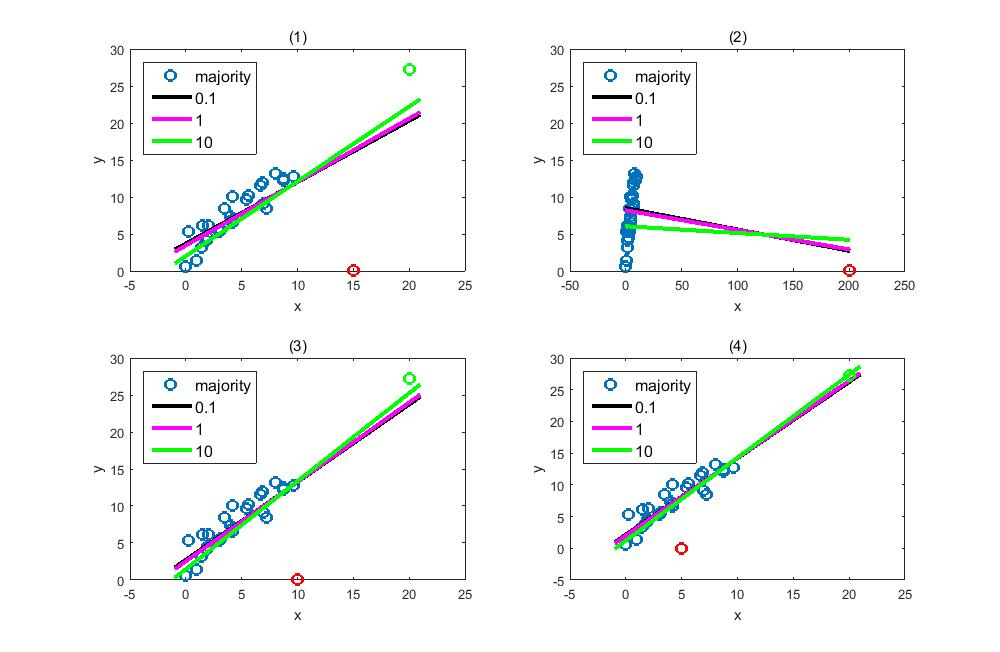
\includegraphics[width=15cm]{C:/Users/okazk_000/Desktop/Spring 2016/CSCI 567/HW1/yeni/HW1/RidgeRegression.jpg}
	\caption{Ridge Regression}
	\label{fig:test}
\end{figure}

\subsubsection{Laplace distribution}
In linear regression model with Gaussian distribution, the points away from centroid of the data points has a very large effect. Laplace distribution may reduce this effect with correct parameters.


\subsubsection{Cook's Distance- Studentized - Leverage Score}
Outlier sample can't be chosen using any of these metrics since in Figure 3 and 4 they all select the leverage point instead of the outlier. Cook's Distance chooses the outlier in Figure 1 and 2.
\begin{figure}[H]%                 use [hb] only if necceccary!
	\centering
	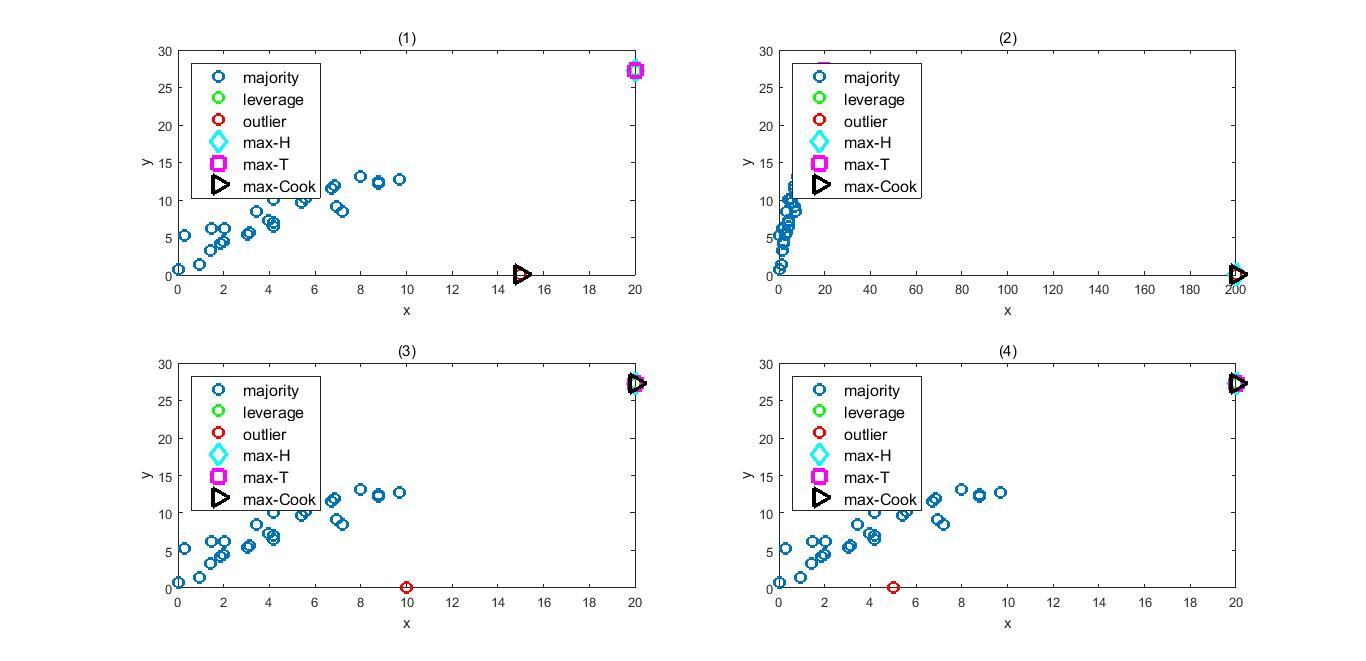
\includegraphics[width=15cm]{C:/Users/okazk_000/Desktop/Spring 2016/CSCI 567/HW1/yeni/HW1/Cook.jpg}
	\caption{Selecting influential samples}
	\label{fig:test}
\end{figure}

\subsection{Classification}
\subsubsection{kNN Classifier Results}
\begin{center}
	\begin{tabular}{|c| c |c |c|} 
		\hline
		k & Training Acc & Validation Acc & Test Acc \\ [0.5ex] 
		\hline
		1 & 0.5835 & 0.6170 & 0.5674 \\ 
		\hline
		3 & 0.9408 & 0.6181 & 0.6084 \\
		\hline
		5 & 0.9173 & 0.6287 & 0.5442 \\
		\hline
		7 & 0.9511 & 0.6404 & 0.5795 \\
		\hline
		9 & 0.9629 & 0.6330 & 0.5879 \\
		\hline
		11 & 0.9598 & 0.6245 & 0.5619 \\
		\hline
		13 & 0.9614 & 0.6181 & 0.5647 \\
		\hline				
		15 & 0.9588 & 0.6181 & 0.5498 \\ [1ex] 
		\hline
	\end{tabular}
\end{center}

\subsubsection{Decision Tree and Performance Comparison}
\begin{center}
	\begin{tabular}{|c| c |c |c|c|c|} 
		\hline
		min Leaf & Split Criteria & Training Acc & Validation Acc & Test Acc\\ [0.5ex] 
		\hline
		1 & Cross Entropy &  0.9829 &  0.6617 & 0.6567    \\ 
		\hline
		2 & Cross Entropy & 0.9829 &  0.6617 & 0.6567   \\ 
		\hline
		3 & Cross Entropy & 0.9829 &  0.6617 & 0.6567  \\ 
		\hline	
		4 & Cross Entropy & 0.9829 &  0.6617 & 0.6567  \\ 
		\hline
		5 & Cross Entropy & 0.9787 & 0.6532  & 0.6567   \\ 
		\hline
		6 & Cross Entropy & 0.9781 & 0.6404  & 0.6567    \\ 
		\hline
		7 & Cross Entropy & 0.9781 & 0.6404  & 0.6567   \\ 
		\hline
		8 & Cross Entropy & 0.9781 & 0.6404 & 0.6567   \\ 
		\hline
		9 & Cross Entropy & 0.9685 & 0.6883 & 0.6149   \\ 
		\hline
		10 & Cross Entropy & 0.9685 & 0.6883 & 0.6149 \\ 
		\hline	
		1 & Gini Index & 0.9793 & 0.6489 & 0.6474   \\ 
		\hline
		2 & Gini Index & 0.9793 & 0.6489 & 0.6474    \\ 
		\hline
		3 & Gini Index & 0.9793 & 0.6489 & 0.6474    \\ 
		\hline	
		4 & Gini Index & 0.9799 & 0.7043 & 0.6474   \\ 
		\hline
		5 & Gini Index & 0.9787 & 0.6957 & 0.6474   \\ 
		\hline
		6 & Gini Index & 0.9781 & 0.6830 & 0.6474   \\ 
		\hline
		7 & Gini Index & 0.9781 & 0.6404 & 0.6567    \\ 
		\hline
		8 & Gini Index & 0.9736 & 0.6404 & 0.6567    \\ 
		\hline
		9 & Gini Index & 0.9594 & 0.6883 & 0.6149  \\ 
		\hline
		10 & Gini Index & 0.9594 & 0.6883 & 0.6149  \\ 
		\hline

	\end{tabular}
\end{center}
		
		
		In the provided dataset, Decision Tree is giving a much better accuracy on Training data. But on validation and testing data, accuracies are close to each other even though Decision Tree is giving a better result in general.
		
		\subsubsection{Decision Boundary}
	\begin{figure}[H]%                 use [hb] only if necceccary!
		\centering
		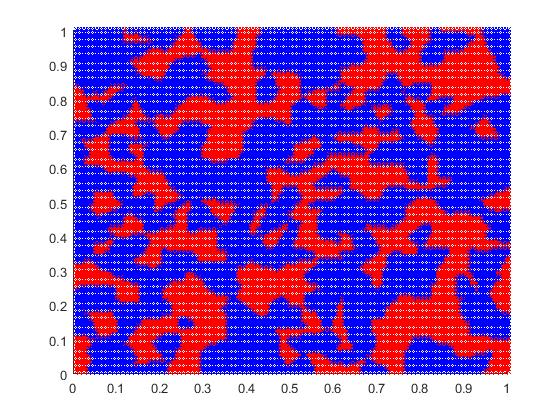
\includegraphics[width=9cm]{C:/Users/okazk_000/Desktop/Spring 2016/CSCI 567/HW1/yeni/HW1/k1.jpg}
		\caption{K = 1}
		\label{fig:test}
	\end{figure}
		\begin{figure}[H]%                 use [hb] only if necceccary!
			\centering
			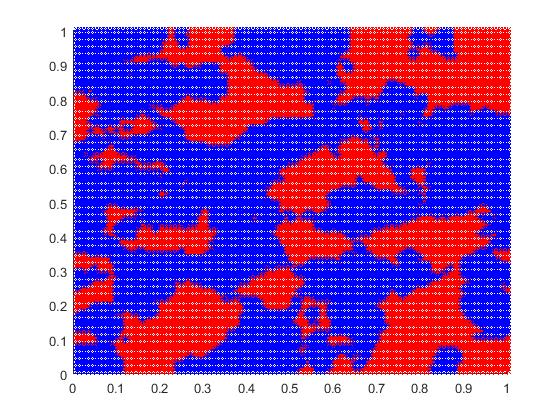
\includegraphics[width=9cm]{C:/Users/okazk_000/Desktop/Spring 2016/CSCI 567/HW1/yeni/HW1/k5.jpg}
			\caption{K = 5}
			\label{fig:test}
		\end{figure}
			\begin{figure}[H]%                 use [hb] only if necceccary!
				\centering
				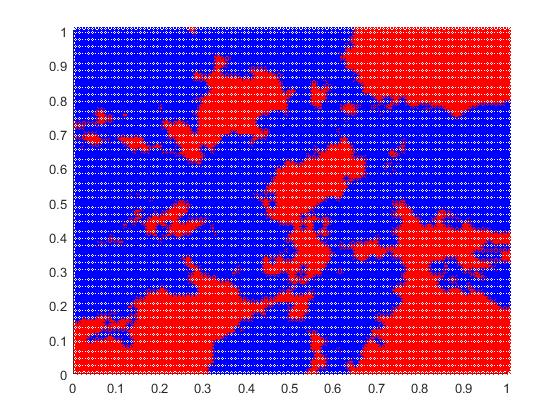
\includegraphics[width=9cm]{C:/Users/okazk_000/Desktop/Spring 2016/CSCI 567/HW1/yeni/HW1/k15.jpg}
				\caption{K = 15}
				\label{fig:test}
			\end{figure}
				\begin{figure}[H]%                 use [hb] only if necceccary!
					\centering
					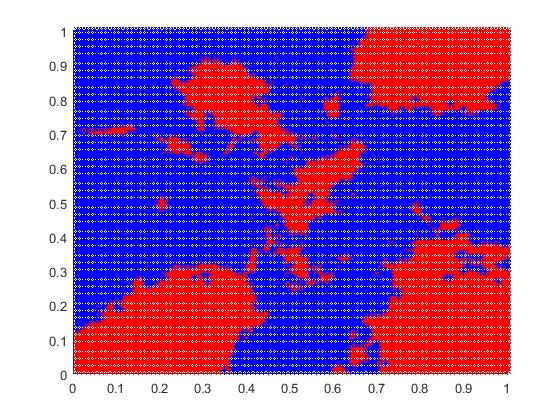
\includegraphics[width=9cm]{C:/Users/okazk_000/Desktop/Spring 2016/CSCI 567/HW1/yeni/HW1/k25.jpg}
					\caption{K = 25}
					\label{fig:test}
				\end{figure}
	While $k$ increases, the decision boundary takes a more flexible and smooth shape. When $k = 1$ decision boundaries only depend on one data point, so it makes a discontinuous decision boundary, with sharp points. 
	
	On the other hand, $k = 25$ has very large areas that belong to the same class, which is way smoother. 
				
	
\end{document}